\documentclass[11pt]{article}

% %%%%%%%%%%%%%%%%%%%%%%%%%%%%%%%%%%%%%%%%%%%%%%%%%%%%%%%%%%%%%%%%%%%%%%%%%%%%%%
% %                                 PACKAGES                                   %
% %%%%%%%%%%%%%%%%%%%%%%%%%%%%%%%%%%%%%%%%%%%%%%%%%%%%%%%%%%%%%%%%%%%%%%%%%%%%%%

% Identify input as UTG-8 format
\usepackage[utf8]{inputenc}

% Style Helvet
\usepackage{setspace}
 \singlespacing
\usepackage[scaled]{helvet}
 \renewcommand\familydefault{\sfdefault}
\usepackage[T1]{fontenc}

% Equations
\usepackage{amsmath}

% Code
\usepackage{listings}
\usepackage[cache=false]{minted}
 \listfiles

% Item Enumeration
\usepackage{enumitem}
% Easy List
\usepackage[ampersand]{easylist}

% Tables
\usepackage{booktabs}
\usepackage{longtable}

% Margins
\usepackage{geometry}
 \geometry{
  a4paper,
  left=25mm,
  top=25mm,
  right=25mm,
  left=25mm
 }

% Images
\usepackage{float}
\usepackage{graphicx}
\usepackage{subcaption}

% Positions and locations
\usepackage{float}

% References
\usepackage{hyperref}

% %%%%%%%%%%%%%%%%%%%%%%%%%%%%%%%%%%%%%%%%%%%%%%%%%%%%%%%%%%%%%%%%%%%%%%%%%%%%%%
% %                                  TITLE                                     %
% %%%%%%%%%%%%%%%%%%%%%%%%%%%%%%%%%%%%%%%%%%%%%%%%%%%%%%%%%%%%%%%%%%%%%%%%%%%%%%

\title{Coursework 1: Experimental Comparison of k-NN and Linear Classification
on the Iris data-set}

\author{
Acereda García, Pablo\\
19043879}

% %%%%%%%%%%%%%%%%%%%%%%%%%%%%%%%%%%%%%%%%%%%%%%%%%%%%%%%%%%%%%%%%%%%%%%%%%%%%%%
% %                               DOCUMENT                                     %
% %%%%%%%%%%%%%%%%%%%%%%%%%%%%%%%%%%%%%%%%%%%%%%%%%%%%%%%%%%%%%%%%%%%%%%%%%%%%%%

\begin{document}

% Title
\maketitle

% This page has been left blank intentionally
\newpage
\vspace*{\fill}
 \begin{center}
This page has been intentionally left blank
 \end{center}
\vspace*{\fill}
\newpage

% Table of contents
\tableofcontents

\newpage

%                            %%%%%%%%%%%%%%
%                             INTRODUCTION
%                            %%%%%%%%%%%%%%
\section{Introduction - Machine Learning and Classification Problems}

Machine learning is the field of study focused on the creation of models to
formulate the answer in regards to a given input. The transformation from a
chaotic input to the desired output takes place by using statistical models and
other fields of study like artificial intelligence (AI).

The process of transformation of a certain input, or training data, to the
desired output, is known as classification problem.

In this process, three main categories can be identified: 
\textit{supervised learning}, \textit{unsupervised learning} and
\textit{reinforcement learning}.

\begin{description}
 
 \item [Supervised Learning] A problem gets this name when the input goes with
  its expected output, so the function obtained to classify new inputs comes
  from labeled training data.
 
 \item [Unsupervised Learning] In this case, no data is labeled. On the 
  contrary, unsupervised search helps finding clusters in data (and therefore 
  labelling them) and correlations in sets of possibly correlated observations.

 \item [Reinforcement Learning] The objective of these algorithms is to maximize
  some notion of cumulative reward, given a certain environment and deciding
  which actions a software agent should take\footnote{''Computer program that
  acts for a user or other program.''}.

\end{description}

The scope of this assignment is not to delve into unsupervised learning; nor is
to go into detail about reinforcement learning (which has not even been 
mentioned in the lectures so far); but to give a description of the implemented
algorithms, the dataset used and to see how those models are applied to the
given dataset.

%                                 DATASET
%                                =========
\subsection{Dataset - Iris Dataset}

Also known as \textit{Iris flower data set} or \textit{Fisher's Iris data set}
\footnote{Name given after Ronald Fishers, who used the dataset in his 
publication in 1936}; is a dataset formed by three flowers from the same 
species: \textbf{Iris flowers}.

According to the original paper, \textit{``All three species were collected in
the Gaspé Peninsula, from the same pasture, picked on the same day and measured
at the same time by the same person with the same apparatus''}.

The three species that the original paper talks about are:

\begin{figure}[H]
 \centering
 \begin{subfigure}{0.32\textwidth}
  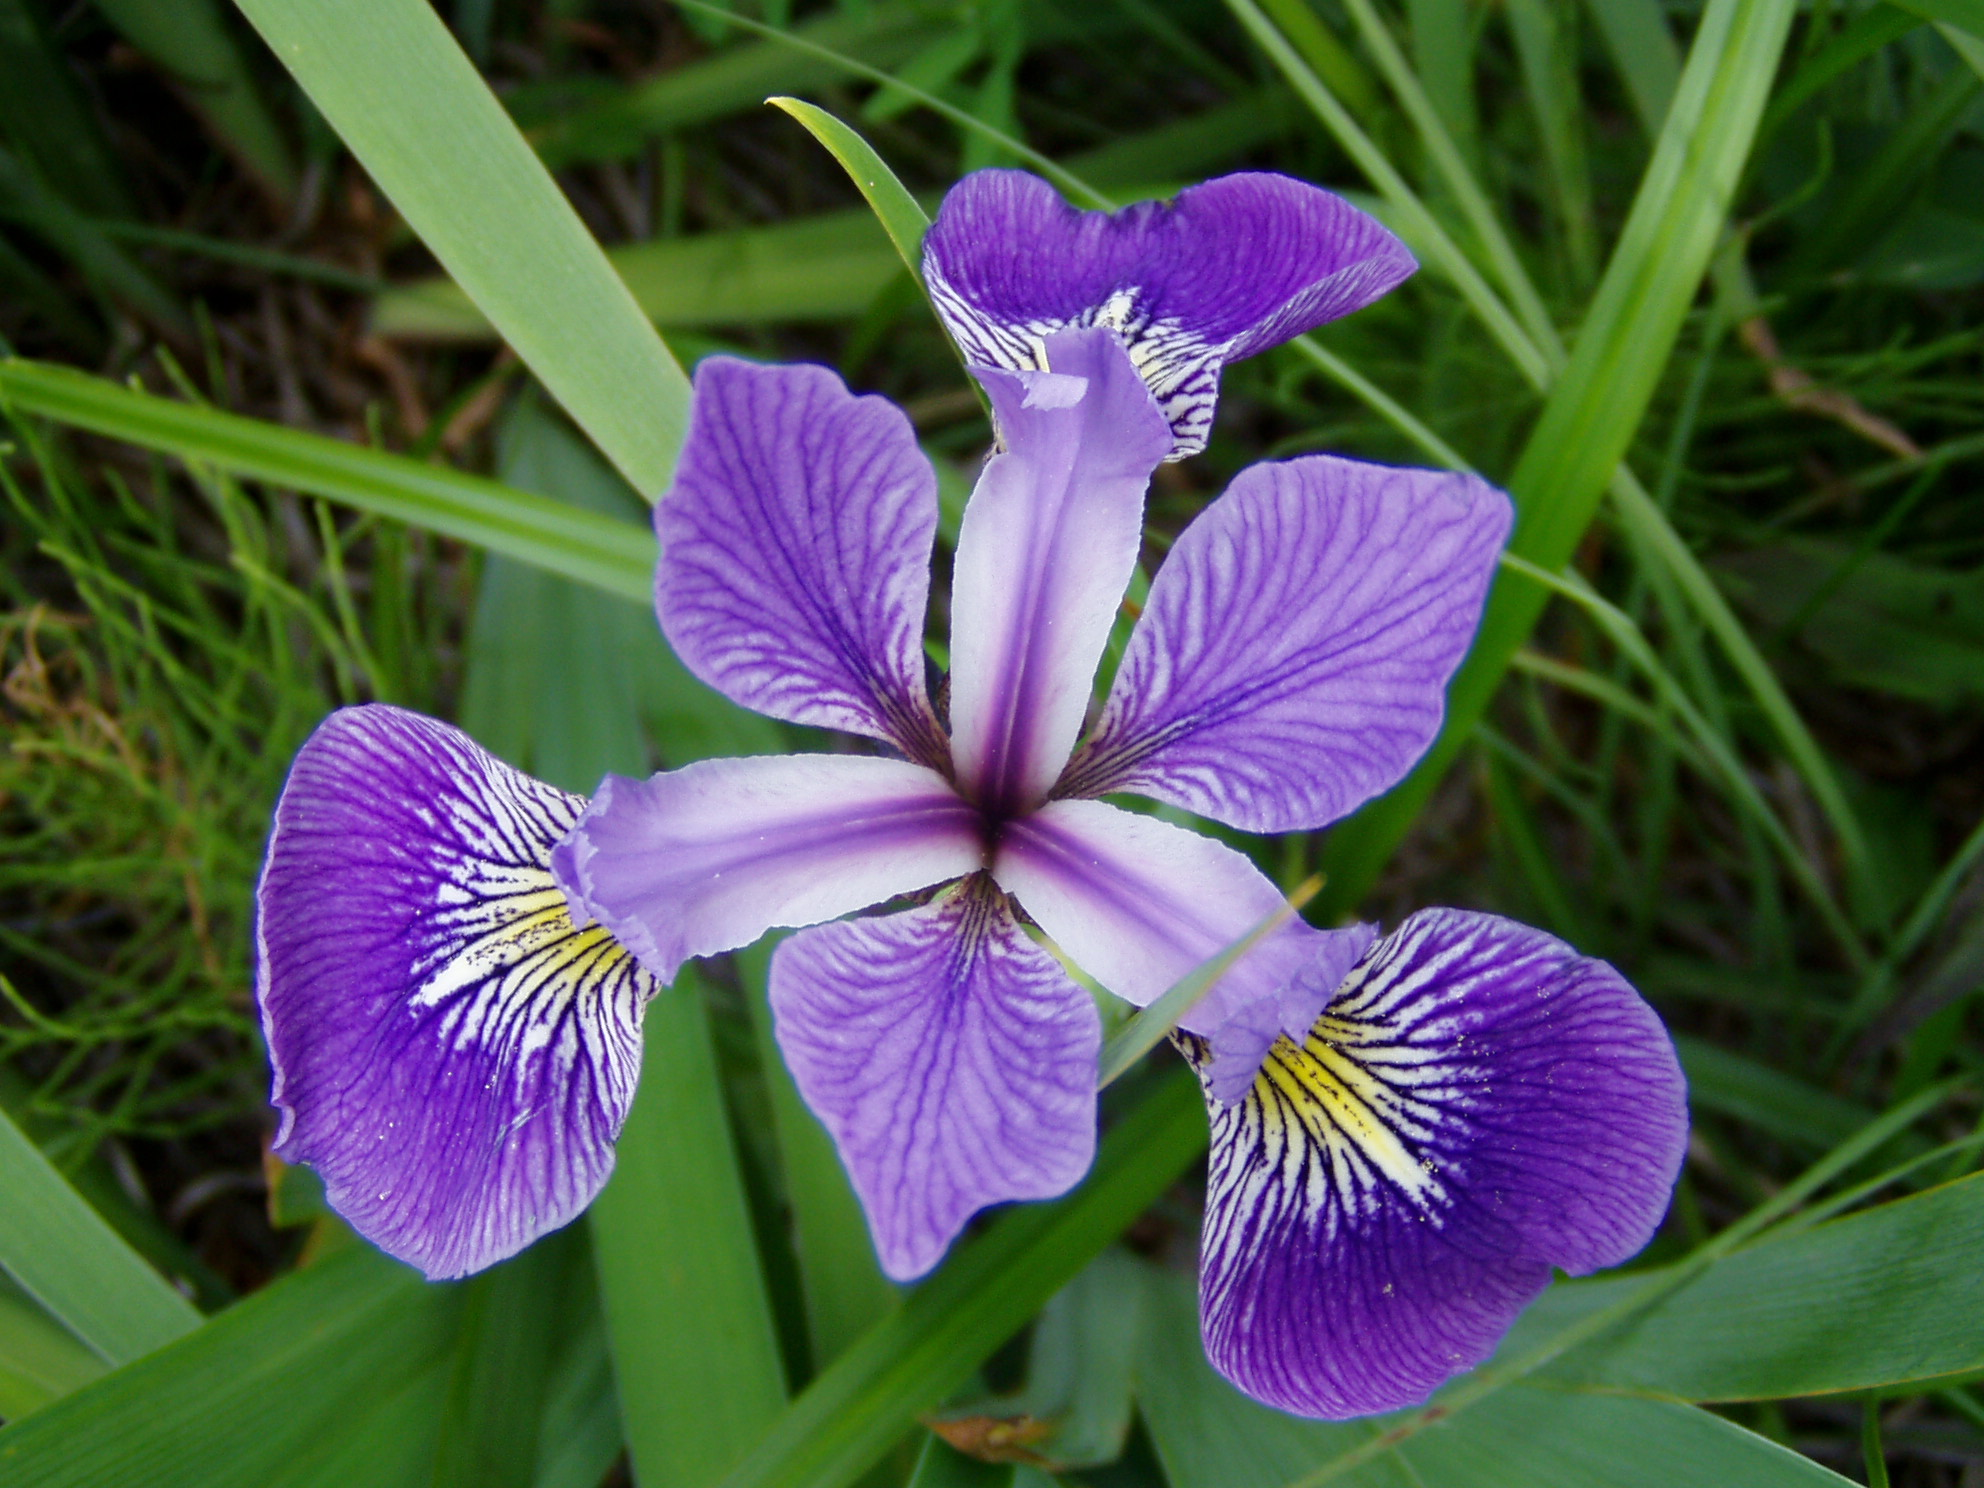
\includegraphics[width=0.9\linewidth]{../images/iris_versicolor.jpg}
  \caption{Iris Versicolor}
 \end{subfigure}
 \begin{subfigure}{0.32\textwidth}
  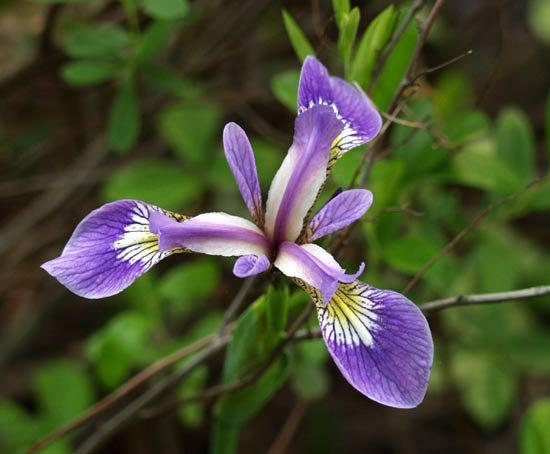
\includegraphics[width=0.9\linewidth]{../images/iris_setosa.jpg}
  \caption{Iris Setosa}
 \end{subfigure}
 \begin{subfigure}{0.32\textwidth}
  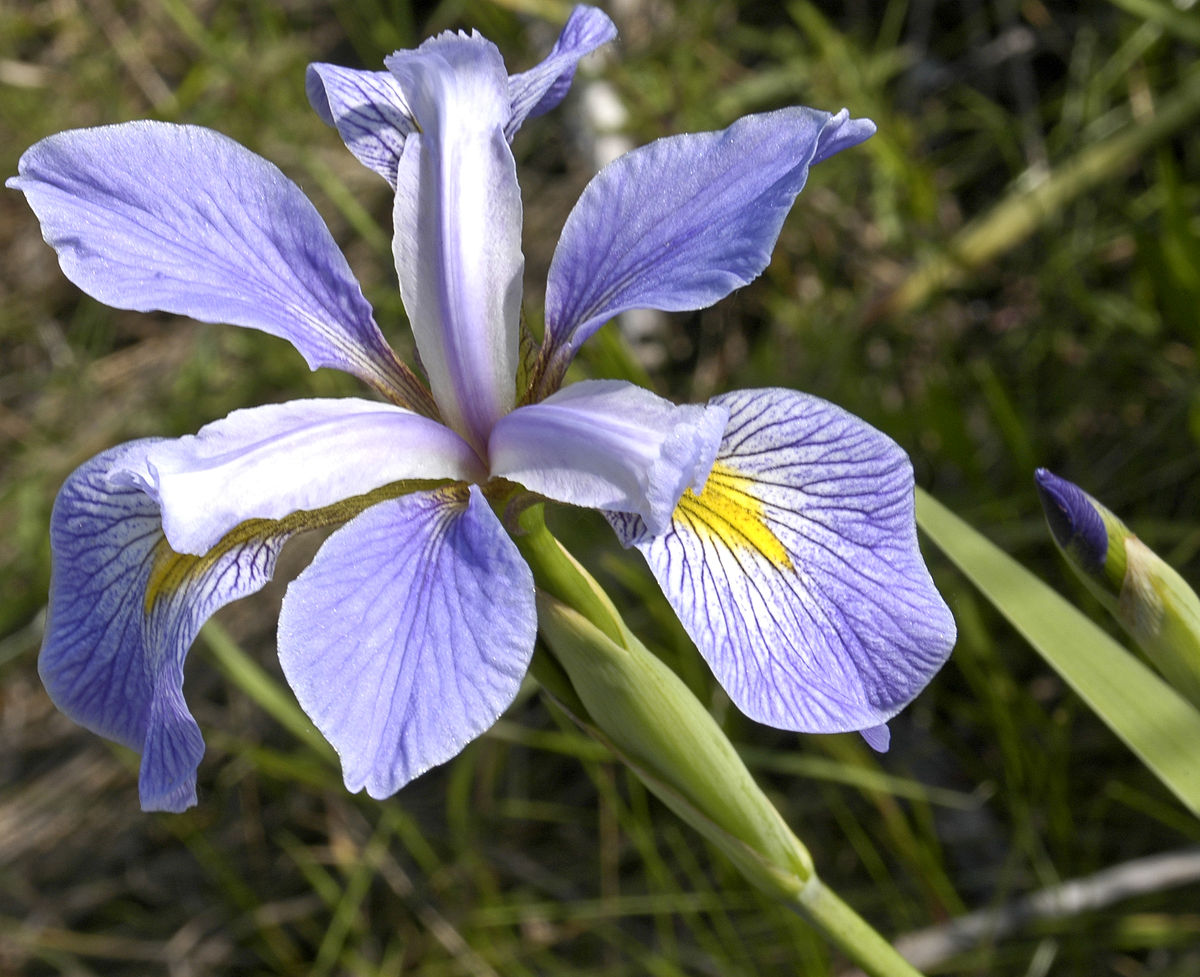
\includegraphics[width=0.9\linewidth]{../images/iris_virginica.jpg}
  \caption{Iris Viginica}
 \end{subfigure}

\end{figure}

There were measured the characteristics of 50 flowers from each particular
specie; taking into account the length and the width from sepals and petals. The
measure unit used for this experiment was centimeters (cm).

\begin{figure}[h]
 \centering
 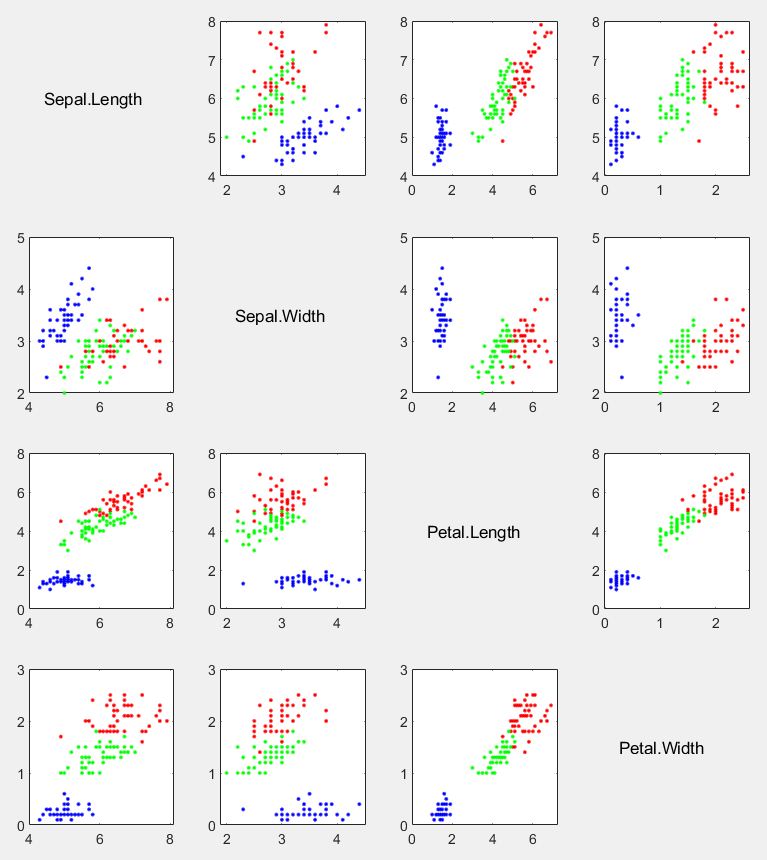
\includegraphics[width=0.65\textwidth, height=10cm]
                 {../images/characteristics.png}
 \caption{Attributes Relation.}
\end{figure}

In this specific project, the Iris Dataset has been used to train and test kNN
and linear classification, randomly ordering the samples to later apply
cross-validation method k-fold.

%                                 MODELS
%                                ========
\subsection{Models - kNN and Linear Classification}

%                            ===== KNN =====
\subsubsection{K-Nearest-Neighbors}

The model kNN has as its objective to classify new inputs by looking at the
\textit{k} closest neighbors. It is possible to understand how it works at a 
glance, when the model is trained by labeled data, it can predict the
class/specie/category of a new sample just by computing the k-nearest neighbors.
That is achieved by using the \textit{Euclidean distance}.

For two dimensions, the formula goes as follows:

\begin{equation}
 \centering
 \sqrt{(x_1 - x_2)^2 + (y_1 - y_2)^2}
\end{equation}

When used in MATLAB, it allows multiple options.

\begin{minted}{matlab}
 Mdl = fitcknn(Tbl, ResponseVarName/formula/Y)
 Mdl = fitcknn(X, Y)
 Mdl = fitcknn(__, Name, Value)
\end{minted}

To ease things, \textit{Tbl and X} are attributes from the samples of data 
used to train the model; \textit{ResponseVarName and Y} are the desired output
for the clusters of samples.

\textit{formula} intends to give an equation on how \textit{Y} depends on the
predictor variables.

A very important argument, or list of arguments, which can be specified after
any of the aforementioned variables is the \textit{Name-Value} Pair Arguments.
They allow to edit properties like what breaks ties in case several samples have
the same properties; the value for k (how many neighbors are selected to decide
the specie), etc.

%                     ===== LINEAR CLASSIFICATION =====
\subsubsection{Linear Classification}

There are actually 2 models which create a linear classification:
\textit{fitclinear} and \textit{fitcecoc}. But, as the first of them does not 
allow multiclass models, - i.e., the one needed for Iris Dataset. Thus, the 
second model is the one being described in this section.

In any case, they both use linear equations to ``separate'' the points from each
species. If a given sample is in the area of a certain species, the model 
decides it belongs to that same class.

\begin{equation}
 \centering
 y = a * bx
\end{equation}

\begin{minted}{matlab}
 Mdl = fitcecoc(Tbl, ResponseVarName/formula/Y)
 Mdl = fitcecoc(X, Y)
 Mdl = fitcecoc(__, Name, Value)

 [Mdl, HyperparameterOptimizationResults] = fitcecoc(__)
\end{minted}

At first sight, both linear and kNN classification have very similar parameters.
The difference can be found, for example, in the pair of arguments
\textit{Name-Value}; which can modify the behaviour of the binary learners, 
design partitions, etc.

There is also one more variable, \textit{HyperparameterOptimizationResults},
which is the description of the cross-validation optimization of
hyperparameters. It is not going to be used, as the cross-validation is to be
implemented manually.

%                                APPLICATION
%                               =============
\subsection{Application - Models to Dataset}

All this theory is very accurate, and also compelling but, how is this going to
help with the Iris Dataset? Fairly simple, by implementing a k-fold
cross-validation which will allow to know the accuracy of the models for the
given data.

With kNN, the more neighbors that are from the same species, the more chances
that input has to be from that species. Varying the significant number of
neighbors, specified by k might also be helpful when it comes to accuracy.

On the other hand, linear classification uses multiclass linear equations to
predict if the given new sample is from one species or not. In this case, no
parameters have been changed.

%                           %%%%%%%%%%%%%%%%%%%
%                            EXPERIMENTAL WORK
%                           %%%%%%%%%%%%%%%%%%%
\section{Experimental Work}

The aforementioned models have been implemented in MATLAB, in addition to other
statistical methods and algorithms in order to predict new samples from the
species \textit{Iris Versicolor}, \textit{Iris Setosa} and \textit{Iris
Virginica}.

The final structure of the algorithm is summarized by the following key points.

\begin{easylist}[enumerate]
 
  & K-fold implementation. Data must me split in k same-sized pieces. Iterating
  on each piece for testing data, and the remaining data used for training.
  
  & Model generation on training data from \textit{Iris Dataset}, previously
  separated by k-fold: \textbf{fitcknn} and \textbf{fitcecoc}.

  & Test models by predicting labels from testing data.

  & Computed error based on the predicted labels and their actual values.

  & Computed the average of all the errors obtained in each iteration performed 
  by the k-fold cross-validation.

  & Data visualization.

\end{easylist}

%                              CROSS-VALIDATION
%                             =================
\subsection{Cross-validation - K-fold}

It works by splitting data in k same-sized parts, and iterating through them, 
so every chunk of data is being used for training and for testing. The models
are trained \textit{k} times, so at the end of the cross-validation it is
computed the average of the error computed in each iteration. A new model
trained with all the samples, should have that average error.

\begin{figure}[h]
 \centering
 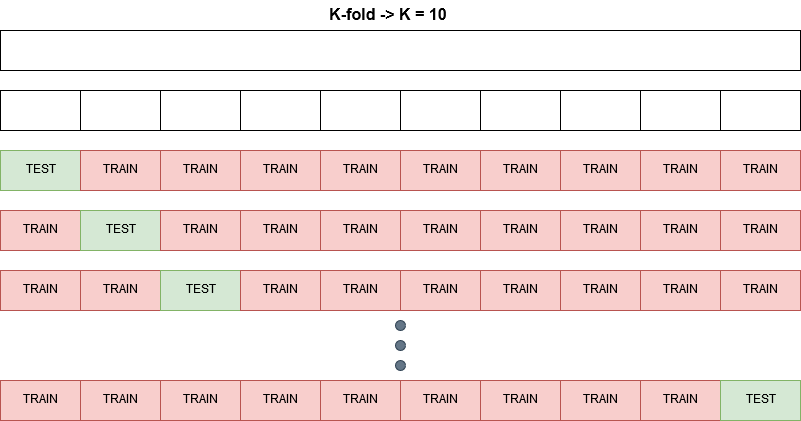
\includegraphics[width=0.75\textwidth]{../diagrams/kfold.png}
 \caption{K-fold cross-validation.}
\end{figure}

\subsection{Modeling and Testing - fitcknn and fitcecoc}

The complexity of this procedure is not inherently very high; once data has been
separated into chunks from the same size, it is only required to specify certain
parameters at most.

\subsection{Error - Cost Function}

The implementation for the problem is the statistical function for the Mean 
Error (ME - \hyperref[me]{\ref{me}}).

\begin{equation}
 \centering
 \frac{1}{N} \sum_{i=1}^{N} {I(a, b)} \label{me}

 \begin{cases}
  I(a, b) = 1, if a \neq b\\
  I(a, b) = 0, if a = b
 \end{cases}
\end{equation}

The usage of any other studied error equation would be absurd. For example,
taking the Mean Squared Error (MSE - \hyperref[mse]{\ref{mse}}):

\begin{equation}
 \frac{1}{N} \sum_{i=1}^{N} {I(a, b)^2} \label{mse}
\end{equation}

To squaring something which has a binary value, 0 or 1\footnote{Should be taken
into account that the predicted label for the sample data can only be right or
wrong}, would actually result in the same value. 

The same thing happens with the Root Mean Squared Error (RMSE - 
\hyperref[rmse]{\ref{rmse}}), only in this case, it would be with the square 
root of the same result that would be obtained with ME (Equation 
\hyperref[me]{\ref{me}}), but in this case proportional to the square root. 
Which, at least for the scope of this project is not really necessary.

\begin{equation}
 \sqrt{\frac{1}{N} \sum_{i=1}^{N} {I(a, b)^2}} \label{rmse}
\end{equation}

There is another function already implemented in MATLAB called 
\textbf{resubLoss}, but it uses weights in the model and other parameters that 
are not available, although it is more accurate, it cannot be implemented with
the known data.

\section{Conclusion}

In brief, two different classification models have been used. Also,
the k-fold cross-validation implementation allows to find the average error rate
of each model.

Looking at the results, the most suitable value for k-fold can be observed: 
surprisingly, it is 100 (after repeating the program execution 20 times). 
The values for k have been changed from 10 to 100 taking steps of 10 at a time. 
Looking at the division scheme, it makes absolute sense; if data is divided into 
100 different pieces, the testing chunks are formed by two elements, which 
rarely gives an error rate higher than 0.

On the other hand, in kNN the value for k in k-fold has been fixed to 10,
changing instead the number of neighbors (from 1 to 150). After looking at 
different executions (once again, 20 runs), the most suitable number of 
neighbors seems to be 17.

The writer has the belief that the selection of the classification method 
depends mainly on the number of samples in the model: if the number of samples 
is too large, kNN classification takes too much time to label new elements. 
On the other hand, if resources and time are not that important, linear 
classification would mean the loss of classification accuracy for most cases 
(kNN looses accuracy after the number of neighbors reaches 80, error rate
escalates).

Finally, the results of the experiment are shown in the next figure
\hyperref[exp]{\ref{exp}}:

\begin{figure}[h]
 \centering
 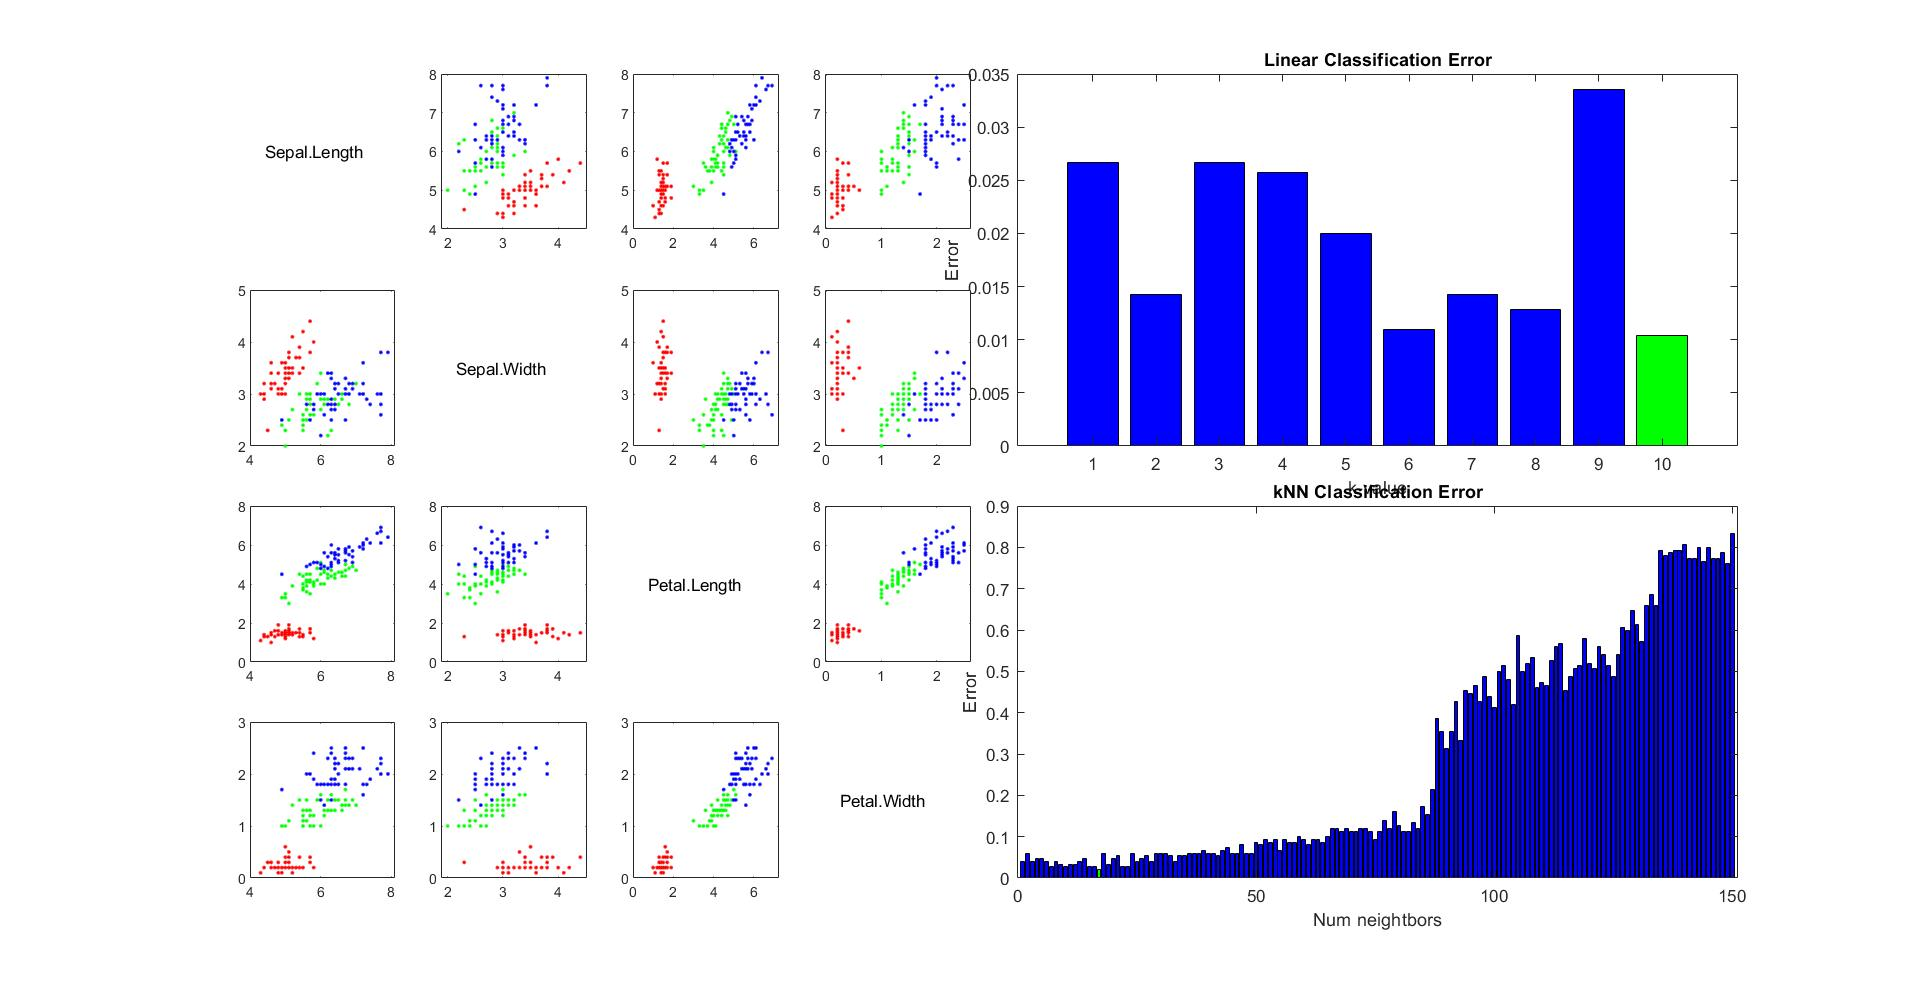
\includegraphics[width=0.7\textwidth]{../experiments/estimation.jpg}
 \caption{To see more experiments go to folder ``./experiments/''.}
 \label{exp}
\end{figure}

\newpage

\section*{Appendix: Code}

The code has been developed in MATLAB. It has been separated in different
chunks separating the models implementations and the experiment itself.

\begin{figure}[h]
 \centering
 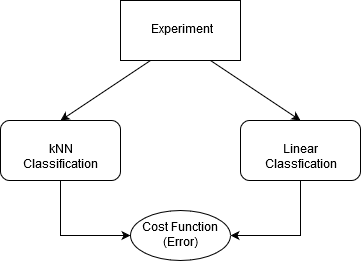
\includegraphics[width=0.8\textwidth]{../diagrams/call_tree.png}
 \caption{Structure of the program - Call Graph.}
\end{figure}

A good practice for a MATLAB script is to have a clean environment.

\begin{minted}{matlab}
% clear variables
% close opened windows
% clean the command windows
%-------------------------------------------------------------------------%
clear variables;
close all;
clc;
%-------------------------------------------------------------------------%
\end{minted}

Afterwards, data is loaded, also creating the folders used for the log files (in
case they do not exist).

\begin{minted}{matlab}
%                              LOAD DATA
%                             ===========
load fisheriris meas species

%                                DATA 
%                               ======

% Want to order samples randomly to apply cross-validation
P = randperm(length(species));

% Data from flower (all in cm):
% { Sepal length | Sepal width | Petal length | Petal width }
X = meas(P, :);

% Class label:
% - Setosa
% - Versicolor
% - Virginica
Y = species(P);

%                             LOGS FOLDERS
%                            ==============

if ~exist("logs/linearlog", 'dir')
   mkdir("logs/linearlog")
   
   disp("Directory logs/linearlog/ has been created.")
end

if ~exist("logs/knnlog", 'dir') 
   mkdir("logs/knnlog")
   
   disp("Directory logs/knnlog/ has been created.")
end
\end{minted}

Afterwards, the functions that perform the linear and the kNN classification are
called: in the case of linear classification, the values for k-folding are
changed as an experiment; in the case of kNN classification, all the possible 
number of neighbors are tested to find the optimal. All these operations are
very time consuming, so some debugging messages are printed (to be aware of the
state of the execution).

\begin{minted}{matlab}
%                                 LINEAR
%                                ========

iterations = 10; 
lin_errs   = zeros(iterations, 2);

disp("Linear classification is executing")

for i = 1 : 1 : iterations
    lin_errs(i, :) = [i * 10,                                           ...
                      linear_classification(10 * i,                     ...
                                            strcat('linearExperimentk', ...
                                                   num2str(10 * i),     ...
                                                   '.log'))];
                      
end

% Minimal error Linear Classification
min_lin_err = min(lin_errs(:, 2));
min_lin_err = lin_errs(:, 2) == min_lin_err;
min_lin_err = lin_errs(min_lin_err == 1, :);

disp(strjoin(["The minimum error for linear classification is ", ...
              num2str(min_lin_err(2)),                           ...
              " for k = ",                                       ...
              num2str(min_lin_err(1))]))
disp("Linear classification has been executed successfully")
disp("")

%                                  KNN
%                                 =====

iterations = 150;
knn_errs   = zeros(iterations, 2); 

disp("kNN classification is about to be executed")

for i = 1 : 1 : iterations
    knn_errs(i, :) = [i,                                         ...
                      knn_classification(10, i,                  ...
                                        strcat('knnExperimentk', ...
                                               num2str(i),       ...
                                               '.log'))];
end

% Minimal error Linear Classification
min_knn_err = min(knn_errs(:, 2));
min_knn_err = knn_errs(:, 2) == min_knn_err;
min_knn_err = knn_errs(min_knn_err == 1, :);

disp(strjoin(["The minimum error for kNN classification is ",   ...
              num2str(min_knn_err(2)),                          ...
              " for k = 10 and the number of neighbors being ", ...
              num2str(min_knn_err(1))]))

disp("kNN classification has been executed successfully")
\end{minted}

Thus, after obtaining all the errors of the different parameters used for each
model, data is plotted to get a more visual way to see the results.

\begin{minted}{matlab}
%                              ==========
%                               PLOTTING
%                              ==========

disp("Plotting data")

% Iris Data Graphs
% Rows
for i = 1 : 1 : 4
    % Columns
    for j = 1 : 1 : 5
        if j <= 4
            % Location in graph
            sp = subplot(4, 8, ((i - 1) * 8 + j));
            % Diagonal             
            if mod(i, 4) ~= mod(j, 4)
                gscatter(X(:, j), X(:, i), Y, 'rgb', '.', 6);
                % Hide legend
                legend('off')
            else
                switch(i)
                    case 1
                        t = "Sepal.Length";
                    case 2
                        t = "Sepal.Width";
                    case 3
                        t = "Petal.Length";
                    case 4
                        t = "Petal.Width";
                    otherwise
                end

                text(0.1, 0.5, t, "Parent", sp); axis off

            end   
            
        else
            % Linear Error
            subplot(4, 8, [5: 8, 13 : 16]);
            bar(lin_errs(:, 1),    lin_errs(:, 2), 'b')
            hold on
            bar(min_lin_err(:, 1), min_lin_err(:, 2), 'g')
            % Title
            title("Linear Classification Error")
            % Labels
            xlabel("k-value")
            ylabel("Error")
            
            % kNN Error
            subplot(4, 8, [21: 24, 29 : 32]);
            bar(knn_errs(:, 1),    knn_errs(:, 2), 'b')
            hold on
            bar(min_knn_err(:, 1), min_knn_err(:, 2), 'g')
            % Title
            title("kNN Classification Error")
            % Labels
            xlabel("Num neightbors")
            ylabel("Error")
            
        end 
    end
end
\end{minted}

In the first classification method, linear classification, it has been tried to 
avoid using too many parameters. As the example developed has a very focused 
scope, the data is loaded again inside the function (although it is not usually 
a good practice, it still is a design choice to ease the developer's workload).

The process after loading the data is fairly simple. The log file that is going
to store every operation is initialized. Then, the model, prediction and error
of the aforementioned operations, are computed with the training data of the
chunk selected by the k-fold crossvalidation (this process is repeated as many
times as the k-fold algorithm stipulates. Finally, the average error of the
model, applying k-folding, is returned.

\begin{minted}{matlab}
% %%%%%%%%%%%%%%%%%%%%%%%%%%%%%%%%%%%%%%%%%%%%%%%%%%%%%%%%%%%%%%%%%%%%%%%%%

% COURSEWORK 1: EXPERIMENTAL COMPARISON OF K-NN AND LINEAR CLASSIFICATION
% ON THE IRIS DATA-SET
% AUTHOR: PABLO ACEREDA
% FILE:   LINEAR_CLASSIFICATION.M

% %%%%%%%%%%%%%%%%%%%%%%%%%%%%%%%%%%%%%%%%%%%%%%%%%%%%%%%%%%%%%%%%%%%%%%%%%

function lin_avg_err = linear_classification(kDiv, filename)

    %                              LOAD DATA
    %                             ===========
    load fisheriris meas species

    %                                DATA 
    %                               ======

    % Want to order samples randomly to apply cross-validation
    P = randperm(length(species));

    % Data from flower (all in cm):
    % { Sepal length | Sepal width | Petal length | Petal width }
    X = meas(P, :);

    % Class label:
    % - Setosa
    % - Versicolor
    % - Virginica
    Y = species(P);

    %                     DATA PARTITIONING INFORMATION
    %                    ===============================

    N    = length(species);
    jump = floor(N / kDiv);

    %                          LOG FILE CREATION
    %                         ===================

    % Moves path to file's path
    cd(fileparts(mfilename('fullpath')));

    % Creates file in case it does not existe
    filename = strcat("logs/linearlog/", filename);
    logFile = fopen(filename, 'w');

    % Writes in log file
    fprintf(logFile,                                           ...
            ['INFO: ',                                         ...
             '==== NEW EXPERIMENT ====\n',                     ...
             'INFO: ',                                         ...
             'Data is going to be divided into %i pieces.\n'], ...
            kDiv);

    % Valid number of divisions
    if kDiv < N

        % Write into log
        fprintf(logFile,                             ...
                ['INFO: ',                           ...
                 'The value for k is valid ',        ...
                 '(k[%i] < number of samples[%i]) ', ...
                 '-> VALID.\n'],                     ...
                kDiv,                                ...
                N);

        %                            VARIABLES
        %                           ===========

        % Column1: Error
        % Column2: Meas
        % Column3: Species Predicted
        % Column4: Species Labeled
        lin = cell(length(kDiv), 4);
        lin(:, 2) = {[100]};

        %                            ========
        %                             K-FOLD
        %                            ========

        for i = 1 : 1 : kDiv

            % Writes in log
            fprintf(logFile,                     ...
                    '\n-- K-FOLD: %i/%i --\n\n', ...
                    i,                           ...
                    kDiv);

            if     i == 1

                testX  = X(       1 : jump, :);
                testY  = Y(       1 : jump, :);
                trainX = X(jump + 1 : end,  :);
                trainY = Y(jump + 1 : end,  :);

            elseif i * jump <= N && i < kDiv 

                testX  = X((i - 1) * jump + 1 : i * jump, :);
                testY  = Y((i - 1) * jump + 1 : i * jump, :);
                trainX = [X(1 : (i - 1) * jump, :) ; ...
                          X(i * jump + 1: end, :)];
                trainY = [Y(1 : (i - 1) * jump, :) ; ...
                          Y(i * jump + 1: end, :)];

            else

                testX  = X((i - 1) * jump + 1 : end, :);
                testY  = Y((i - 1) * jump + 1 : end, :);
                trainX = X(1                  : (i - 1) * jump     , :);
                trainY = Y(1                  : (i - 1) * jump     , :);

            end

            %                         ========
            %                          LINEAR
            %                         ========

            %                           MODEL
            Mdl_linear = fitcecoc(trainX, trainY, ...
                                  'ClassNames', ["setosa",     ...
                                                 "versicolor", ...
                                                 "virginica"]);
            %                          TESTING
            pred_lin = predict(Mdl_linear, testX);
            %                           ERROR
            err_lin = costfunction(testY, pred_lin) / length(testY);

            % Writes in log
            fprintf(logFile,                          ...
                    ['// LINEAR \\\\\n',              ...
                     'Prediction for training: %s\n', ...
                     'Actual values:           %s\n', ...
                     'Error: %f\n'],                  ...
                    strjoin(pred_lin),                ...
                    strjoin(testY),                   ...
                    err_lin);

            %                      ERROR STORAGE
            lin(i, :) = {[err_lin] [trainX] [pred_lin] [testY]};

            % Log: extra separation
            fprintf(logFile, '\n');

        end
    % ------------------------------------------------------------------- %

        lin_avg_err = sum(cell2mat(lin(:, 1))) / length(lin);

        fprintf(logFile,                                                ...
                ['\n===============================================\n', ...
                'Linear Mean Error: %f'],                               ...
                lin_avg_err);

    else
        fprintf(logFile,                             ...
                ['ERROR: ',                          ...
                 'The value for k is too large ',    ...
                 '(k[%i] < number of samples[%i]) ', ...
                 '-> VALID.\n'],                     ...
                kDiv,                                ...
                N);
    end

    % Writes everything in log
    fclose(logFile);

    lin_avg_err;

end
\end{minted}

The aforementioned pattern is repeated once again for the kNN classification,
this time in a separated function.

\begin{minted}{matlab}
% %%%%%%%%%%%%%%%%%%%%%%%%%%%%%%%%%%%%%%%%%%%%%%%%%%%%%%%%%%%%%%%%%%%%%%%%%

% COURSEWORK 1: EXPERIMENTAL COMPARISON OF K-NN AND LINEAR CLASSIFICATION
% ON THE IRIS DATA-SET
% AUTHOR: PABLO ACEREDA
% FILE:   KNN_CLASSIFICATION.M

% %%%%%%%%%%%%%%%%%%%%%%%%%%%%%%%%%%%%%%%%%%%%%%%%%%%%%%%%%%%%%%%%%%%%%%%%%

function knn_avg_err = knn_classification(kDiv, k_value, filename)

    %                              LOAD DATA
    %                             ===========
    load fisheriris meas species 

    %                                DATA 
    %                               ======

    % Want to order samples randomly to apply cross-validation
    P = randperm(length(species));

    % Data from flower (all in cm):
    % { Sepal length | Sepal width | Petal length | Petal width }
    X = meas(P, :);

    % Class label:
    % - Setosa
    % - Versicolor
    % - Virginica
    Y = species(P);

    %                     DATA PARTITIONING INFORMATION
    %                    ===============================

    N    = length(species);
    jump = floor(N / kDiv);

    %                          LOG FILE CREATION
    %                         ===================

    % Moves path to file's path
    cd(fileparts(mfilename('fullpath')));

    % Creates file in case it does not existe
    filename = strcat("logs/knnlog/", filename);
    % Open file 
    logFile = fopen(filename, 'w');

    % Writes in log file
    fprintf(logFile,                                           ...
            ['INFO: ',                                         ...
             '==== NEW EXPERIMENT ====\n',                     ...
             'INFO: ',                                         ...
             'Data is going to be divided into %i pieces.\n'], ...
            kDiv);

    % Valid number of divisions
    if kDiv <= N

        % Write into log
        fprintf(logFile,                             ...
                ['INFO: ',                           ...
                 'The value for k is valid ',        ...
                 '(k[%i] < number of samples[%i]) ', ...
                 '-> VALID.\n'],                     ...
                kDiv,                                ...
                N);

        %                            VARIABLES
        %                           ===========

        % Column1: Error
        % Column2: Meas
        % Column3: Species Predicted
        % Column4: Species Labeled
        knn = cell(length(kDiv), 4);
        knn(:, 2) = {[100]};

        %                            ========
        %                             K-FOLD
        %                            ========

        for i = 1 : 1 : kDiv

            % Writes in log
            fprintf(logFile,                     ...
                    '\n-- K-FOLD: %i/%i --\n\n', ...
                    i,                           ...
                    kDiv);

            if     i == 1

                testX  = X(       1 : jump, :);
                testY  = Y(       1 : jump, :);
                trainX = X(jump + 1 : end,  :);
                trainY = Y(jump + 1 : end,  :);

            elseif i * jump <= N && i < kDiv 

                testX  = X((i - 1) * jump + 1 : i * jump, :);
                testY  = Y((i - 1) * jump + 1 : i * jump, :);
                trainX = [X(1 : (i - 1) * jump, :); ...
                          X(i * jump + 1: end, :)];
                trainY = [Y(1 : (i - 1) * jump, :); ...
                          Y(i * jump + 1: end, :)];

            else

                testX  = X((i - 1) * jump + 1 : end, :);
                testY  = Y((i - 1) * jump + 1 : end, :);
                trainX = X(1                  : (i - 1) * jump     , :);
                trainY = Y(1                  : (i - 1) * jump     , :);

            end

            %                          =====
            %                           KNN
            %                          =====

            %                          MODEL
            Mdl_knn = fitcknn (trainX, trainY, 'NumNeighbors', k_value);
            %                         TESTING
            pred_knn = predict(Mdl_knn, testX);
            %                          ERROR
            err_knn = costfunction(testY, pred_knn) / length(testY);

            % Writes in log
            fprintf(logFile,                          ...
                    ['** KNN (k=%i) **\n',            ...
                     'Prediction for training: %s\n', ...
                     'Actual values:           %s\n', ...
                     'Error: %f\n'],                  ...
                      k_value,                        ...
                      strjoin(pred_knn),              ...
                      strjoin(testY),                 ...
                      err_knn);

            %                      ERROR STORAGE
            knn(i, :) = {[err_knn] [trainX] [pred_knn] [testY]};

            % Log: extra separation
            fprintf(logFile, '\n');
        end
    % ------------------------------------------------------------------- %

        knn_avg_err = sum(cell2mat(knn(:, 1))) / length(knn);

        fprintf(logFile,                                                ...
                ['\n===============================================\n', ...
                'kNN Mean Error: %f'],                                  ...
                knn_avg_err);

    else
        fprintf(logFile,                             ...
                ['ERROR: ',                          ...
                 'The value for k is too large ',    ...
                 '(k[%i] < number of samples[%i]) ', ...
                 '-> VALID.\n'],                     ...
                kDiv,                                ...
                N);
    end

    % Writes everything in log
    fclose(logFile);
    
    knn_avg_err;

end
\end{minted}

Finally, the cost function implemented to compute the mean error of the
predictions made by the models.

\begin{minted}{matlab}
function cost = costfunction(known, estimated)
    cost = sum(int8(not(strcmp(known, estimated))));
end
\end{minted}

\end{document}

